\pagenumbering{arabic}
\setcounter{page}{1}
%% Los cap'itulos inician con \chapter{T'itulo}, estos aparecen numerados y
%% se incluyen en el 'indice general.
%%
%% Recuerda que aqu'i ya puedes escribir acentos como: 'a, 'e, 'i, etc.
%% La letra n con tilde es: 'n.

\chapter{Introducci'on}
%%
%%Existen dos tipos de citas bibliograf'icas: usa \verb|\citep{..}| para
%%citas en \emph{par'entesis} y \verb|\citet{..}| para citas
%%en el \emph{texto}. Por ejemplo, estudios reciente han mostrado nuevos e
%%interesantes modelos que se pueden aplicar para reformular teor'ias
%%f'isicas~\citep{NewCam97}. Mientras que, el trabajo de \citet{Rofl06} fue
%%considerado muy divertido por una significativa fracci'on de la comunidad
%%de investigadores. Tambi'en es posible citar a varios trabajos en una sola
%%referencia \citep{Lamport86,Knuth84}.

%%Estos comandos para producir citas bibliograficas son provistos por
%%el paquete \textsf{natbib}. Para obtener m'as informaci'on, consulta la
%%documentaci'on de ese paquete~\citep{doc:natbib}. Por su parte, en
%%la documentaci\'on de \textsf{geometry} puedes encontrar detalles
%%adicionales sobre el sistema para ajustar los m'argenes del
%%documento~\citep{doc:geometry}. Lo que sigue
%%es un mont'on de texto sin sentido en lat'in que utilizaremos para llenar
%%algunas p'aginas.


El desarrollo de controladores es una constante que va de mano con el crecimiento econ'omico y tecnol'ogico
de los pueblos y sus industrias; impulsando avances en los procesos industriales con el proposito de fomentar competitividad para los paises en materia tecnol'ogica \citep{odanilo}.

Al desarrollar controladores que funcionen de la manera m'as adecuada en sistemas lineales y no lineales
representa en si un reto, en especial desde el punto de vista academico, al tratar de acoplar la utilidad de 
los controladores, con la seguridad que deben presentar, y lo confiables que deben ser a la hora de su implementaci'on  \citep{odanilo}.

	Existe una simple razon por la cual el ``P'endulo'' es tan utilizado en investigaci'on, es su din'amica no lineal, que permite comprender el comportamiento de sistemas mas complejos desde el punto de vista de su linealidad y din'amica, como lo son los sectores de transporte, telecomunicaciones, aeron'autica; con lo que los controladores son facilmente aplicables a estos sistemas \citep{odanilo}.
	
En el presente trabajo se realizar'a la implementaci'on de un controlador con t'ecnicas de tiempo real montada en un arduino a trav'es de una red de campo (basada en protocolos de comunicaci'on CAN multi-nodo); donde los datos de monitoreo ser'an presentados cada cierto tiempo en la HMI desarrollada para el mismo prop'osito.

%% Los cap'itulos inician con \chapter{T'itulo}, estos aparecen numerados y
%% se incluyen en el 'indice general.
%%
%% Recuerda que aqu'i ya puedes escribir acentos como: 'a, 'e, 'i, etc.
%% La letra n con tilde es: 'n.

\section{Objetivos}

%\prefacesection{Objetivos}
\subsection{Objetivo Principal:}
			\begin{itemize}
			\item Desarrollar e implementar el sistema de control del p'endulo invertido a trav'es de una red de campo.\\
			\end{itemize}
				 
\subsection{Objetivos Espec'ificos:}
			\begin{itemize}
			\item Revisar bibliograf'ia y documentos acerca del estado del arte referente al control por red.
			\item	Determinar los requisitos y par'ametros necesarios para realizar el dise'no del sistema de control en base a las caracter'isticas de la planta, y a su funci'on de transferencia.
			\item	Dise'nar y probar  el sistema de control del p'endulo a trav'es de software de simulaci'on. 
			\item	Dise'nar la HMI para adquisici'on de datos y supervisi'on.
			\item	Implementar el sistema de control y probarlo para condiciones reales de trabajo.
			\end{itemize} 

\section{Antescedentes}

El sistema de p'endulo es uno de los m'as factibles de resolver dentro del mundo f'isico; ya que de el parten varios problemas que se ponen de manifiesto para los sistemas de control\citep{BoteOrtega}.

El mod'elo matem'atico que se traslada de la realidad a lo abstracto de la f'isica del p'endulo, presenta una formulaci'on basada en ecuaciones diferenciales, que se asemejan en muchos casos a otros sistemas reales m'as o menos complejos, dentro de varios sectores tecnol'ogicos, como puede ser el control seguro de una planta qu'imica o un sistema de vuelo de aeronaves. Por ende, e estudio de este sistema sirve como punto de partida para el desarrollo de controladores mas especializados para sistemas m'as complejos\citep{BoteOrtega}.


Basados ya en ese punto, el p'endulo invertido presenta una enorme variedad de problemas que lo hacen uno de los sistemas m'as concretos y utiles a la hora del ensayo de leyes de control, en las 'ultimas d'ecadas. Los primeros p'endulos nacieron en los 70, y a'un despu'es de tantos a'nos se sigue utilizando el p'endulo como caso de estudio de y de investigaci'on\citep{BoteOrtega}. 

\section{Problema}


En teor'ia de control uno de los problemas mas conocidos, cl'asicos e importantes es el asi llamado ``P'endulo Invertido''. Y tiene como aplicaciones desde el control de estabilidad de gr'uas hasta el modelamiento de la bipedestaci'on humana \citep{Legaspi12}; y no est'a dem'as decir que este tipo de sistemas esta presente en varias universidades, como por ejemplo la Universidad Nacional de Colombia, La Universidad Complutense de Madrid, La Universidad Aut'onoma de Puebla, entre muchas otras al rededor del mundo; por lo que de primera mano se puede ver que al rededor del mundo utilizan estre problema f'isico como un sistema base para el desarrollo de controladores en investigaciones acad'emicas.

Es accesible desde el punto de vista acad'emico y de control relativamente f'acil, en 'el se pueden observar caracter'isticas de sistemas de lazo abierto y cerrado \citep{Legaspi12}.

Hay que tener presente que dentro de la UTN y especialmente en la facultad de ingenier'ia, no se cuenta con m'odulos ni plantas basados en hardware y software abierto orientados al uso did'actico o como base para el desarrollo de investigaci'on cient'ifica. \\


\begin{figure}[h] %h posicion de la grafica
\centering
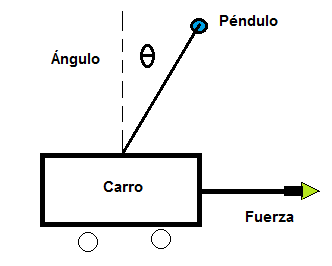
\includegraphics[scale=0.70]{pendulo1}
\caption{Diagrama simple del P'endulo.}
\label{fig:pendulo1}
\end{figure}

\section{Justificaci'on}

Al conseguir los objetivos del proyecto, se desea demostrar que es posible controlar un sistema de control de din'amica r'apida a trav'es de una red de campo (basada en una capa f'isica o de enlace).

Por las caracter'isticas ampliamente estudiadas del p'endulo invertido, siendo 'este una planta no lineal de segundo orden, y considerando que muchos sistemas f'isicos reales son similares, esta planta se convierte en un sistema 'util para el ensayo de soluciones de control, as'i como  para el desarrollo de sistemas de control m'as eficientes.

Este proyecto permitir'a cumplir dos metas: 
\begin{itemize}
	\item Afianzar el conocimiento te'orico adquirido por el estudiante a trav'as de la implementaci'on de sistemas reales.
 \item Servir como plataforma para el ensayo de nuevas soluciones de control obtenidas a trav'as de la investigaci'on.
\end{itemize}

\section{Alcance}


La construcci'on del p'endulo constituye un proyecto impulsado por el grupo de investigaci'on en control y optimizaci'on de la UTN en el que se podr'a probar diferentes t'ecnicas de dise'no de controladores tales como control 'optimo y control por posicionamiento de polos (espacio de estados);  implementaci'on de observadores y observadores 'optimos. Todo esto en base a funciones de transferencia sustentadas matem'aticamente que podr'ian comprender el modelado de retardos de propagaci'on y procesamiento. Se pondra a prueba el sistema con un controlador basado en t'ecnicas de estado de espacios; con lo cual se validar'a la funcionalidad de todo el sistema.


El control a implementarse en el p'endulo se realizar'a a trav'es de varios sistemas microprocesados comunicados mediante una red de campo (control distribuido).
Adem'as la planta contar'a con una HMI (interfaz humano-m'aquina) implementada en un ordenador, con el fin de establecer un sistema de supervisi'on y adquisici'on de datos del p'endulo para un posterior an'alisis off-line. Todo los sistemas es basar'an en software y hardware libre.

\section{Datos generales}
\subsection{Sistema Mec'anico}
El sistema mec'anico as'i como los componentes del mismo est'an descritos a detalle en la tesis que precede a 'este trabajo; conformado de: una mesa, un sistema de rieles que permiten la movilidad, un carro, un sistema eje-p'endulos, sensores de posici'on y un sistema de transmisi'on de fuerza con un motor acoplado.

\subsection{Sistema Electr'onico y de Control}
En breves rasgos el sistema electr'onico esta compuesto por placas 4 ``Arduinos Uno'' montadas en una red CAN. Cada nodo a detalle ser'a explicado en posteriores cap'itulos; pero b'asicamente los nodos 1 y 2 obtendra datos de los sensores los procesar'a y convertir'a pertinentemente a las unidades adecuadas; el nodo central o nodo 0 procesar'a estos datos y con ellos calcular'a una acci'on de control que ser'a enviada al nodo 3 donde se la convertir'a en voltaje para accionar el motor acoplado al sistema.